\documentclass[titlepage, 12pt, a4paper]{article}

%The "polyglossia" package allows the use of Greek fonts alongside English ones
\usepackage{polyglossia}
    \newfontfamily\greekfont[Script=Greek]{Linux Libertine O}
    \newfontfamily\greekfontsf[Script=Greek]{Linux Libertine O}
    \setdefaultlanguage{greek}
    \setotherlanguage{english}

% The "amsmath" package allows the inclusion of mathematica symbols in
% the LaTeX document.
\usepackage{amsmath}

% The "array" package allows the center allignment of columns with wrapped
% content.
\usepackage{array}
    \newcolumntype{P}[1]{>{\centering\arraybackslash}p{#1}}

%  The "ulem" package allows strikethrough effect in text.
\usepackage{ulem}

% The "graphicx" package allows insertion of images
\usepackage{graphicx}

% The "ragged2e" package allows justified text (pliri stixoisi)
\usepackage[document]{ragged2e}




\begin{document}
\begin{titlepage}
%\title{\Huge Υψηλές Τάσεις Ι\\ \huge Αναφορά Εργαστηρίου\\ \huge Εργαστηριακή άσκηση 2}
%\author{
%    Ευστρατίου Ευστράτιος ΑΕΜ 10489
%   \and
%   Κουτσικάκης Δημήτριος ΑΕΜ 10532
%   \and
%   Μανακίδης Παύλος ΑΕΜ 10436
%   \and
%   Παναγιωτίδης Γεώργιος ΑΕΜ 10369
%   \and
%   Παναπακίδης Δημήτριος ΑΕΜ 9298
%}
\begin{center}
    \vspace*{1cm}
            
    \Huge
    \textbf{Υψηλές Τάσεις Ι}
            
    \vspace{0.5cm}
    \LARGE
    Εργαστηριακή Αναφορά
            
    \vspace{2.5cm}
    \LARGE     
    Ομάδα 1\\
    \Large
    \vspace{0.2cm}
    Ευστρατίου Ευστράτιος ΑΕΜ 10489\\
    \vspace{0.2cm}
    Κουτσικάκης Δημήτριος ΑΕΜ 10532\\
    \vspace{0.2cm}
    Μανακίδης Παύλος ΑΕΜ 10436\\
    \vspace{0.2cm}
    Παναγιωτίδης Γεώργιος ΑΕΜ 10369\\
    \vspace{0.2cm}
    Παναπακίδης Δημήτριος ΑΕΜ 9298
            
    \vfill
    \Large        
    Εργαστηριακή Άσκηση 2\\
    Μετασχηματιστές Δοκιμής και Φαινόμενο Ferranti
            
    \vspace{0.8cm}
            
    \large
    Τμήμα Ηλεκτρολόγων Μηχανικών και Μηχανικών Υπολογιστών ΑΠΘ\\
    Δευτέρα 13 Νοεμβρίου 2023
            

\end{center}
\date{Χειμερινό Εξάμηνο 2023-2024}
\end{titlepage}

\justifying

\vspace{1cm}
\section*{ΜΕΤΑΣΧΗΜΑΤΙΣΤΕΣ ΔΟΚΙΜΗΣ ΚΑΙ ΦΑΙΝΟΜΕΝΟ FERRANTI}
\vspace{0.3cm}
\subsection*{Ερώτημα 1.1 - Υπολογισμός $U_1'$}

Οι τρεις Μ/Σ δοκιμής TEO 100/10, 2x220V/100kV/220V, 5kVA, 4\% που χρησιμοποιούνται στην εργαστηριακή άσκηση έχουν έκαστος \textbf{Λόγο Μετασχηματισμού  $w$}$ =454.54$, ο οποίος προκύπτει ως εξής:

\[w = \frac{V_n \text{\footnotesize  δευτερεύοντος}}{V_n \text{\footnotesize  πρωτεύοντος}} = \frac{100kV}{220V} = 454.54\]

όπου "\textbf{$V_n$}" η ονομαστική τάση ενός τυλίγματος του Μ/Σ.

\vspace{0.2cm}
Όταν αυτοί χρησιμοποιούνται ένας μόνος ή δύο συνδεδεμένοι κατα βαθμίδες ή τρεις συνδεδεμένοι κατά βαθμίδες, στην πλευρά της ΥΤ παρουσιάζουν ονομαστική τάση $100kV$, $200kV$ και $300kV$ αντίστοιχα (\textit{όπως φαίνεται και στον Πίνακα 3.1 του φυλλαδίου του εργαστηρίου}). Τότε οι συνολικές διατάξεις έχουν αντίστοιχα Λόγους Μετασχηματισμού:

\[w_1 = \frac{100kV}{220V} = 454.54\]

\[w_2 = \frac{200kV}{220V} = 909.09\]

\[w_3 = \frac{300kV}{220V} = 1363.63\]

\vspace{0.2cm}
Αν οι Μ/Σ θεωρηθούν \textbf{ιδανικοί} και λειτουργούν \textbf{εν κενώ}, για δοθείσες τάσεις πρωτεύοντος οι τάσεις στην έξοδο της διάταξης ($U_1'$) ισούνται με τις ανηγμένες τάσεις του πρωτεύοντος στo δευτερεύον και προκύπτουν όπως παρακάτω:

\vspace{0.2cm}
\centering
\begin{tabular}{|c|c|c|} \hline 
         Αριθμός Βαθμίδων Μ/Σ Δοκιμής & Τάση Εισόδου $U_1$ & Τάση Εξόδου  $U_1'$\\ \hline 
        1 & $30V$ & $13.63kV$\\ \hline
        2 & $15V$ & $13.63kV$\\ \hline
        3 & $10V$ & $13.63kV$\\ \hline
    \end{tabular}

\vspace{0.2cm}
\justifying
Παρακάτω παρατίθενται αναλυτικά τις πράξεις:

\[U_1' = U_1\cdot w_1 = 30\cdot 454.54 = 13.63kV\]
\[U_1' = U_1\cdot w_2 = 15\cdot 909.09= 13.63kV\]
\[U_1' = U_1\cdot w_3 = 10\cdot 1363.63 = 13.63kV\]

\subsection*{Ερωτήματα 1.2 και 1.3 - Υπολογισμός $U_{2F}$ και Ανύψωσης Τάσης}

Η φόρτιση των Μ/Σ δοκιμής είναι σχεδόν πάντα χωρητική λόγω της εσωτερικής χωρητικότητας τους και των διαφόρων δοκιμίων που συνδέονται στην έξοδό τους, τα οποία έχουν χωρητικό χαρακτήρα). Η τάση εξόδου τους $U_{2F}$ (τάση δευτερέυοντος τυλίγματος) σε αυτές τις περιπτώσεις υπολογίζεται προσεγγιστικά από τη σχέση:

\begin{equation}
U_{2F} \approx U_1'\cdot \frac{1}{1-u}
\end{equation}

\vspace{0.2cm}
όπου με $u$ συμβολίζεται η συνολική ανά μονάδα τάσης βραχυκύκλωσης της διάταξης (\textbf{λαμβάνοντας υπόψιν και την επίδραση του φορτίου}).

\vspace{0.2cm}
Τότε, συγκεκριμένα για λειτουργία \textbf{εν κενώ}, για δοθείσες τάσεις πρωτεύοντος οι τάσεις στην έξοδο της διάταξης ($U_{2F}$) προκύπτουν όπως παρακάτω:

\vspace{0.2cm}
\centering
\begin{tabular}{|P{2.8cm}|P{3cm}|P{2cm}|P{1.8cm}|P{1.8cm}|P{1.2cm}|} \hline 
         Αριθμός Βαθμίδων Μ/Σ Δοκιμής & Τάση Βραχυκύκλωσης ($u$) & Τάση Εισόδου ($U_1$) & Τάση Εξόδου ($U_1'$) & Τάση Εξόδου ($U_{2F}$) & $\epsilon(\%)$\\ \hline 
        1 & 4\% & $30V$ & $13.63kV$ & $14.21kV$ & $4.2\%$\\ \hline
        2 & 7\% & $15V$ & $13.63kV$ & $14.66kV$ & $7.6\%$\\ \hline
        3 & 11\% & $10V$ & $13.63kV$ & $15.32kV$ & $12.4\%$\\ \hline
    \end{tabular}

\vspace{0.5cm}
\justifying
Η ανύψωση τάσης $\epsilon(\%)$ προκύπτει ως εξής:

\[\epsilon(\%) = \frac{U_{2F}-U_1'}{U_1'}\]

και οφείλεται στην παρουσία \textbf{παρασιτικών χωρητικοτήτων} στην διάταξη. 

\vspace{0.2cm}
Αξίζει να σημειωθεί το γεγονός ότι οι χωρητικότητες αυτές έχουν πολύ μεγαλύτερη σύνθετη αντίσταση (συγκ. αντίδραση) από την ισοδύναμη αυτεπαγωγή των διατάξεων - ειδάλλως θα υπήρχε πτώση τάσης αντί για ανύψωση.
\newpage
\subsection*{Ερώτημα 2 - Αποτελέσματα Εργαστηριακών Μετρήσεων}

\vspace{0.2cm}
Συνδέθηκαν στην έξοδο των διατάξεων Μ/Σ δοκιμής:
\begin{enumerate}
    \item Αρχικά ένας πυκνωτής $100pF$
    \item Έπειτα δύο πυκνωτές $100pF$ και $1300pF$ \textbf{παράλληλα}.
\end{enumerate}
Αυτοί οι πυκνωτές μπορούν να θεωρηθούν παράλληλα συνδεδεμένοι με την παρασιτική χωρητικότητα ($C_i$) της διάταξης, όπως φαίνεται στην παρακάτω φωτογραφία.\\

\begin{figure}[h]
    \centering
    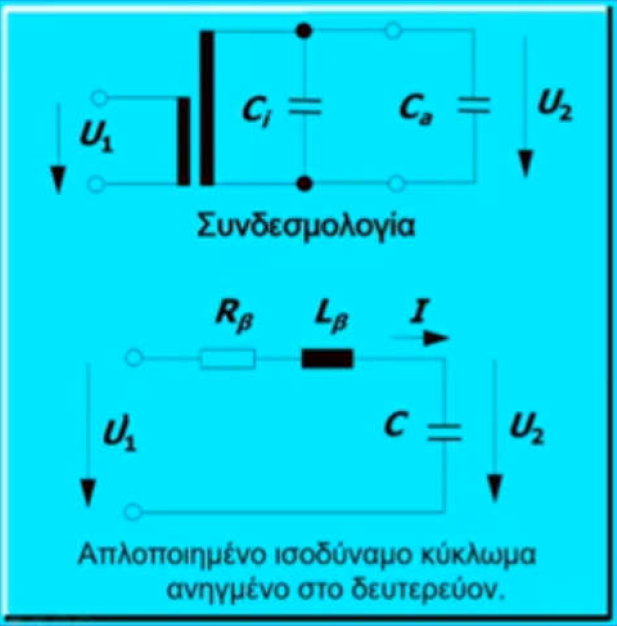
\includegraphics[width=7.5cm]{Images/Test_Transformer.png}
    \caption{Μ/Σ δοκιμής με χωρητικό φορτίο}
   % \label{fig:galaxy}
\end{figure}

Η συνολική ισοδύναμη χωρητικότητα $C$ μπορεί να υπολογιστεί ως εξής:

\[C_a = C_{100pF} +  C_{1300pF}\]
\[ C = C_i + C_a = C_i + C_{100pF} + C_{1300pF}\]

\vspace{0.2cm}
Σε αυτό το σημείο να σημειωθεί ότι η εξίσωση $(1)$ μπορεί να γραφεί και ως εξής:

\begin{equation}
U_{2F} \approx U_1'\cdot \frac{1}{1-u} \approx U_1'\cdot \frac{1}{1-\omega^2L_{\beta
}C}
\end{equation}

\vspace{0.2cm}
Παρατηρούμε ότι αύξηση της συνολικής χωρητικότητας ($C$) συνεπάγεται \textbf{αύξηση} και της τάσης εξόδου ($U_{2F}$) της διάταξης του Μ/Σ δοκιμής.

\vspace{0.2cm}
Αυτό επιβεβαιώνεται και από τις πειραματικές μετρήσεις στο εργαστήριο, οι οποίες συνοψίζονται στον παρακάτω πίνακα.

\vspace{0.5cm}
\centering
\begin{tabular}{|P{2.2cm}|P{1.5cm}|P{1.5cm}|P{2.1cm}|P{2.1cm}|P{1.5cm}|P{1.5cm}|} \hline 
         Αριθμός Βαθμίδων Μ/Σ Δοκιμής & Τάση Εισόδου ($U_1$) & Τάση Εξόδου ΕΝ ΚΕΝΩ & Πειραματική Τάση Εξόδου ($100pF$) & Πειραματική Τάση Εξόδου ($1300pF$) & $\epsilon(\%)$ $(100pF)$ & $\epsilon(\%)$ $(1300pF$)\\ \hline 
        1 & $30V$ & $14.21kV$ & $14.0kV$ & $14.5kV$ & $0\%$ & $3.6\%$\\ \hline
        2 & $15V$ & $14.66kV$ & $14.3kV$ & $18.9kV$ & $2.1\%$ & $35\%$\\ \hline
        3 & $10V$ & $15.32kV$ & $15.2kV$ & $22.5kV$ & $8.6\%$ & $61\%$\\ \hline
    \end{tabular}

\vspace{0.5cm}
\justifying
όπου η  ανύψωση τάσης $\epsilon(\%)$ προκύπτει ως εξής:

\[\epsilon(\%) = \frac{U_{2F}-U_{2F-100pF}}{U_{2F-100pF}}, \hspace{0.5cm} U_{2F}: \textit{Η πειραματική τάση εξόδου των διατάξεων}\]
\newpage
\subsection*{Ερώτημα 3 - Σχολιασμός Μετρήσεων και Υπολογισμών}

Μέσα από τη διεξαγωγή της εργαστηριακής άσκησης επιβεβαιώθηκε και πειραματικά ότι όσο εντονότερη είναι η συνολική χωρητική φόρτιση, τόσο μεγαλύτερη είναι και η ανύψωση της τάσης εξόδου ($U_{2F}$) της διάταξης του Μ/Σ δοκιμής (Φαινόμενο Ferranti).

\vspace{0.2cm}
Σε κάθε περίπτωση, όπως φαίνεται από τις πειραματικές μετρήσεις, η προσθήκη του δεύτερου πυκνωτή παράλληλως ενίσχυσε τη συνολική χωρητική φόρτιση και αύξησε την τάση εξόδου ($U_{2F}$) της διάταξης.

\vspace{0.2cm}
Το ίδιο παρατηρείται και κατά την προσθήκη βαθμίδας στη διάταξη των Μ/Σ δοκιμής. Οι Μ/Σ δοκιμής έχουν από την κατασκευή τους μια εσωτερική χωρητικότητα. Επομένως, η προσθήκη νέας βαθμίδας Μ/Σ θα προσθέσει επιπλέον χωρητικότητα στη διάταξη, γεγονός το οποίο εξηγεί και την αύξηση της ανύψωσης τάσης $\epsilon (\%)$ μετά την προσθήκη νέας βαθμίδας, δηλαδή την ανύψωση της τάσης εξόδου ($U_{2F}$).
Όσον αφορά βέβαια την ανηγμένη τάση του πρωτεύοντος στο δευτερεύον ($U_1'$), κατά την πειραματική διαδικασία, με κατάλληλη μεταβολή των τυλιγμάτων του αυτομετασχηματιστή του εργαστηρίου η τάση αυτή παρέμεινε κατά το δυνατόν σταθερή.

\vspace {0.2cm}
Μετά από αυτή την ανάλυση, βέβαια, θα περίμενε κανείς η τάση εξόδου \textbf{εν κενώ} να ήταν χαμηλότερη της τάσης με φορτίο τον πυκνωτή των $100pF$. Το γεγονός ότι κάτι τέτοιο δεν παρατηρείται μπορεί να εξηγηθεί, καθώς η τιμή της "Τάσης Εξόδου ΕΝ ΚΕΝΩ" δεν είναι πειραματική, αλλά θεωρητική. Στην πράξη οι τάσεις βραχυκύκλωσης ($u$) των Μ/Σ δοκιμής αναμένεται να είναι \textbf{μικρότερες} και έτσι η "Τάση Εξόδου ΕΝ ΚΕΝΩ" \textbf{μικρότερη} από την Τάση Εξόδου $U_{2F}$ (βλ. εξίσωση ($1$)).

\vspace{0.2cm}
Ολοκληρώνοντας, ο υπολογισμός της τάσης εξόδου $U_{2F}$ (τάση δευτερεύοντος τυλίγματος) του Μ/Σ δοκιμής μέσω του γινομένου της τάσης πρωτεύοντος επί το λόγο μετασχηματισμού $w$ μπορεί να οδηγήσει σε σημαντικά σφάλματα ιδιαίτερα στις περιπτώσεις μεγάλης χωρητικής φόρτισης Μ/Σ δοκιμής με τάση βραχυκύκλωσης μεγάλης τιμής.

\end{document}
